\documentclass[1p]{elsarticle_modified}
%\bibliographystyle{elsarticle-num}

%\usepackage[colorlinks]{hyperref}
%\usepackage{abbrmath_seonhwa} %\Abb, \Ascr, \Acal ,\Abf, \Afrak
\usepackage{amsfonts}
\usepackage{amssymb}
\usepackage{amsmath}
\usepackage{amsthm}
\usepackage{scalefnt}
\usepackage{amsbsy}
\usepackage{kotex}
\usepackage{caption}
\usepackage{subfig}
\usepackage{color}
\usepackage{graphicx}
\usepackage{xcolor} %% white, black, red, green, blue, cyan, magenta, yellow
\usepackage{float}
\usepackage{setspace}
\usepackage{hyperref}

\usepackage{tikz}
\usetikzlibrary{arrows}

\usepackage{multirow}
\usepackage{array} % fixed length table
\usepackage{hhline}

%%%%%%%%%%%%%%%%%%%%%
\makeatletter
\renewcommand*\env@matrix[1][\arraystretch]{%
	\edef\arraystretch{#1}%
	\hskip -\arraycolsep
	\let\@ifnextchar\new@ifnextchar
	\array{*\c@MaxMatrixCols c}}
\makeatother %https://tex.stackexchange.com/questions/14071/how-can-i-increase-the-line-spacing-in-a-matrix
%%%%%%%%%%%%%%%

\usepackage[normalem]{ulem}

\newcommand{\msout}[1]{\ifmmode\text{\sout{\ensuremath{#1}}}\else\sout{#1}\fi}
%SOURCE: \msout is \stkout macro in https://tex.stackexchange.com/questions/20609/strikeout-in-math-mode

\newcommand{\cancel}[1]{
	\ifmmode
	{\color{red}\msout{#1}}
	\else
	{\color{red}\sout{#1}}
	\fi
}

\newcommand{\add}[1]{
	{\color{blue}\uwave{#1}}
}

\newcommand{\replace}[2]{
	\ifmmode
	{\color{red}\msout{#1}}{\color{blue}\uwave{#2}}
	\else
	{\color{red}\sout{#1}}{\color{blue}\uwave{#2}}
	\fi
}

\newcommand{\Sol}{\mathcal{S}} %segment
\newcommand{\D}{D} %diagram
\newcommand{\A}{\mathcal{A}} %arc


%%%%%%%%%%%%%%%%%%%%%%%%%%%%%5 test

\def\sl{\operatorname{\textup{SL}}(2,\Cbb)}
\def\psl{\operatorname{\textup{PSL}}(2,\Cbb)}
\def\quan{\mkern 1mu \triangleright \mkern 1mu}

\theoremstyle{definition}
\newtheorem{thm}{Theorem}[section]
\newtheorem{prop}[thm]{Proposition}
\newtheorem{lem}[thm]{Lemma}
\newtheorem{ques}[thm]{Question}
\newtheorem{cor}[thm]{Corollary}
\newtheorem{defn}[thm]{Definition}
\newtheorem{exam}[thm]{Example}
\newtheorem{rmk}[thm]{Remark}
\newtheorem{alg}[thm]{Algorithm}

\newcommand{\I}{\sqrt{-1}}
\begin{document}

%\begin{frontmatter}
%
%\title{Boundary parabolic representations of knots up to 8 crossings}
%
%%% Group authors per affiliation:
%\author{Yunhi Cho} 
%\address{Department of Mathematics, University of Seoul, Seoul, Korea}
%\ead{yhcho@uos.ac.kr}
%
%
%\author{Seonhwa Kim} %\fnref{s_kim}}
%\address{Center for Geometry and Physics, Institute for Basic Science, Pohang, 37673, Korea}
%\ead{ryeona17@ibs.re.kr}
%
%\author{Hyuk Kim}
%\address{Department of Mathematical Sciences, Seoul National University, Seoul 08826, Korea}
%\ead{hyukkim@snu.ac.kr}
%
%\author{Seokbeom Yoon}
%\address{Department of Mathematical Sciences, Seoul National University, Seoul, 08826,  Korea}
%\ead{sbyoon15@snu.ac.kr}
%
%\begin{abstract}
%We find all boundary parabolic representation of knots up to 8 crossings.
%
%\end{abstract}
%\begin{keyword}
%    \MSC[2010] 57M25 
%\end{keyword}
%
%\end{frontmatter}

%\linenumbers
%\tableofcontents
%
\newcommand\colored[1]{\textcolor{white}{\rule[-0.35ex]{0.8em}{1.4ex}}\kern-0.8em\color{red} #1}%
%\newcommand\colored[1]{\textcolor{white}{ #1}\kern-2.17ex	\textcolor{white}{ #1}\kern-1.81ex	\textcolor{white}{ #1}\kern-2.15ex\color{red}#1	}

{\Large $\underline{10_{109}~(K10a_{93})}$}

\setlength{\tabcolsep}{10pt}
\renewcommand{\arraystretch}{1.6}
\vspace{1cm}\begin{tabular}{m{100pt}>{\centering\arraybackslash}m{274pt}}
\multirow{5}{120pt}{
	\centering
	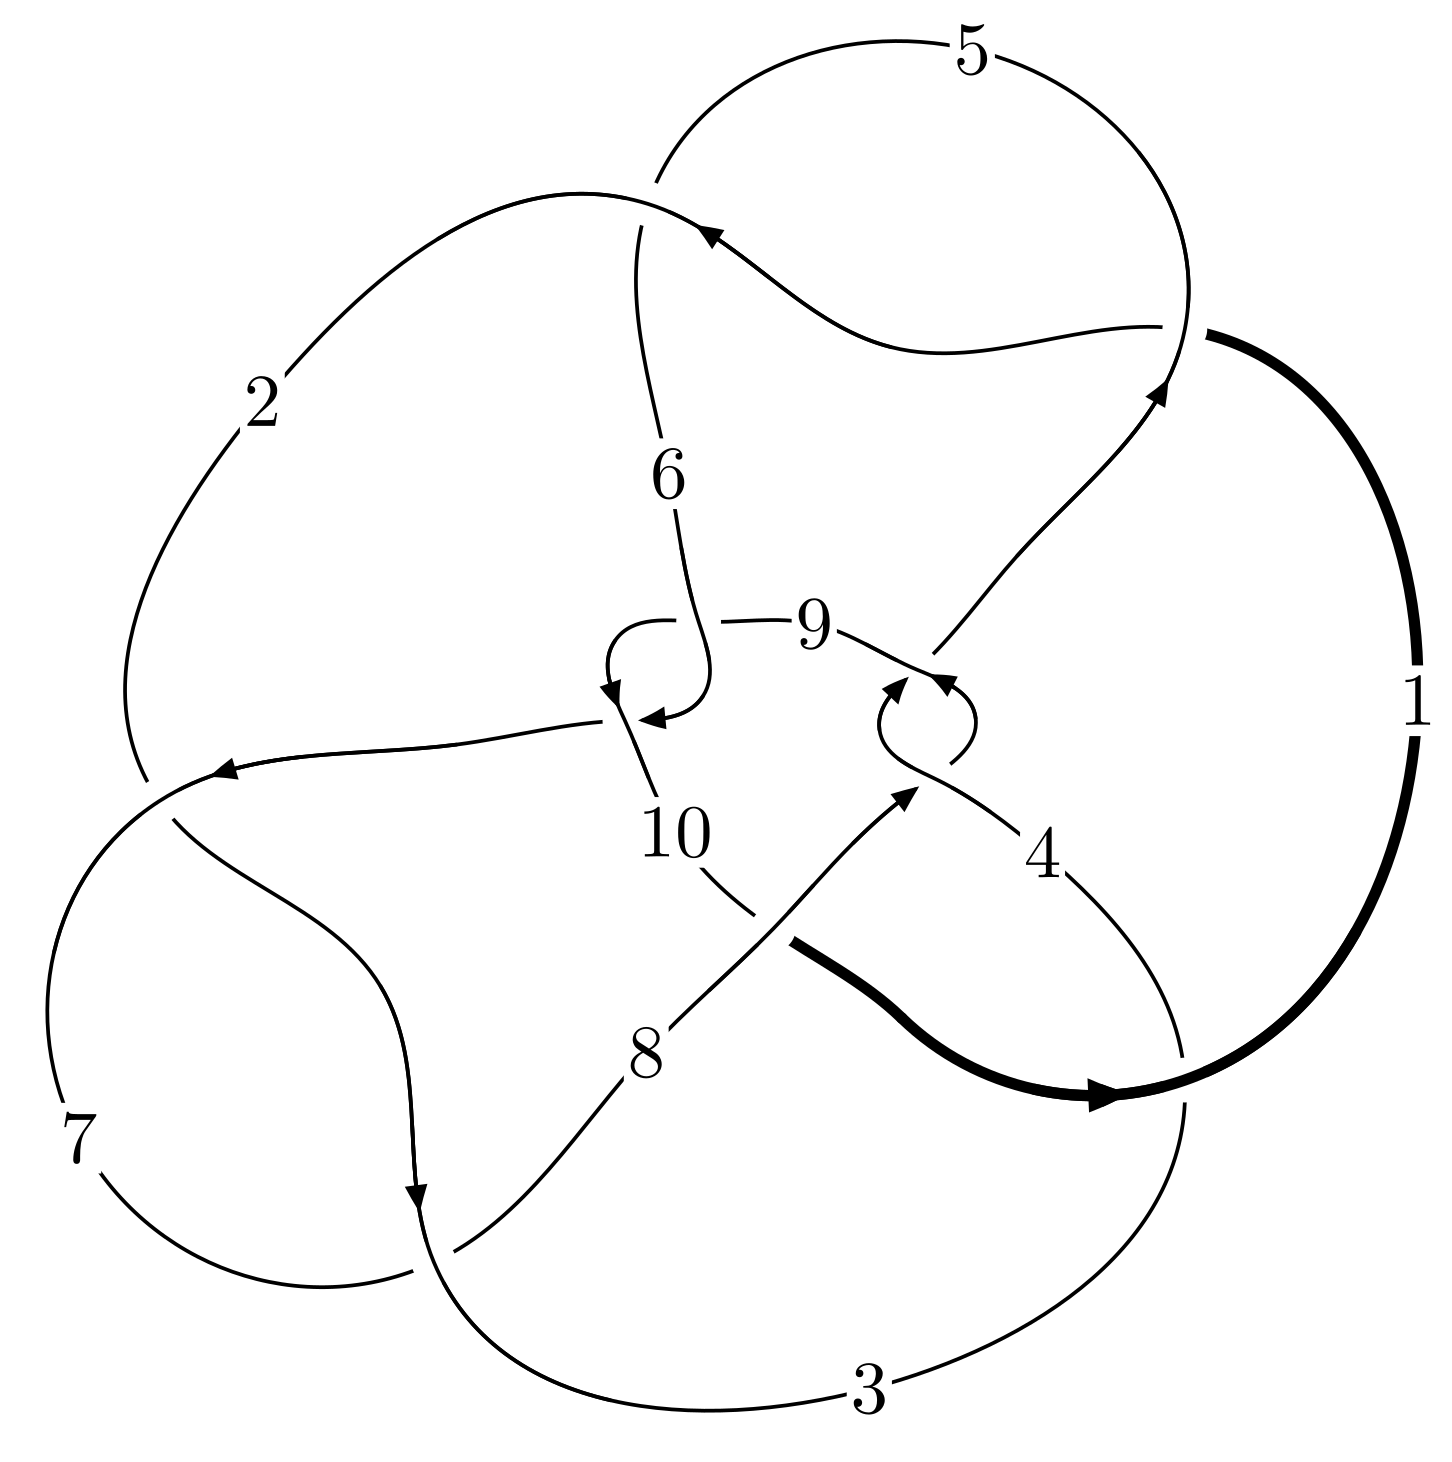
\includegraphics[width=112pt]{../../../GIT/diagram.site/Diagrams/png/193_10_109.png}\\
\ \ \ A knot diagram\footnotemark}&
\allowdisplaybreaks
\textbf{Linearized knot diagam} \\
\cline{2-2}
 &
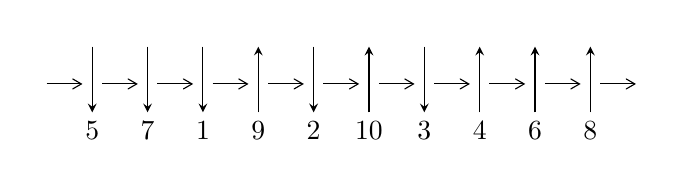
\begin{tikzpicture}[x=20pt, y=17pt]
	% nodes
	\node (C0) at (0, 0) {};
	\node (C1) at (1, 0) {};
	\node (C1U) at (1, +1) {};
	\node (C1D) at (1, -1) {5};

	\node (C2) at (2, 0) {};
	\node (C2U) at (2, +1) {};
	\node (C2D) at (2, -1) {7};

	\node (C3) at (3, 0) {};
	\node (C3U) at (3, +1) {};
	\node (C3D) at (3, -1) {1};

	\node (C4) at (4, 0) {};
	\node (C4U) at (4, +1) {};
	\node (C4D) at (4, -1) {9};

	\node (C5) at (5, 0) {};
	\node (C5U) at (5, +1) {};
	\node (C5D) at (5, -1) {2};

	\node (C6) at (6, 0) {};
	\node (C6U) at (6, +1) {};
	\node (C6D) at (6, -1) {10};

	\node (C7) at (7, 0) {};
	\node (C7U) at (7, +1) {};
	\node (C7D) at (7, -1) {3};

	\node (C8) at (8, 0) {};
	\node (C8U) at (8, +1) {};
	\node (C8D) at (8, -1) {4};

	\node (C9) at (9, 0) {};
	\node (C9U) at (9, +1) {};
	\node (C9D) at (9, -1) {6};

	\node (C10) at (10, 0) {};
	\node (C10U) at (10, +1) {};
	\node (C10D) at (10, -1) {8};
	\node (C11) at (11, 0) {};

	% arrows
	\draw[->,>={angle 60}]
	(C0) edge (C1) (C1) edge (C2) (C2) edge (C3) (C3) edge (C4) (C4) edge (C5) (C5) edge (C6) (C6) edge (C7) (C7) edge (C8) (C8) edge (C9) (C9) edge (C10) (C10) edge (C11) ;	\draw[->,>=stealth]
	(C1U) edge (C1D) (C2U) edge (C2D) (C3U) edge (C3D) (C4D) edge (C4U) (C5U) edge (C5D) (C6D) edge (C6U) (C7U) edge (C7D) (C8D) edge (C8U) (C9D) edge (C9U) (C10D) edge (C10U) ;
	\end{tikzpicture} \\
\hhline{~~} \\& 
\textbf{Solving Sequence} \\ \cline{2-2} 
 &
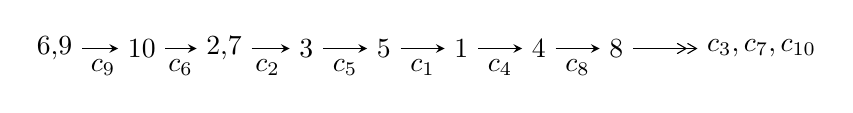
\begin{tikzpicture}[x=28pt, y=7pt]
	% node
	\node (A0) at (-1/8, 0) {6,9};
	\node (A1) at (1, 0) {10};
	\node (A2) at (33/16, 0) {2,7};
	\node (A3) at (25/8, 0) {3};
	\node (A4) at (33/8, 0) {5};
	\node (A5) at (41/8, 0) {1};
	\node (A6) at (49/8, 0) {4};
	\node (A7) at (57/8, 0) {8};
	\node (C1) at (1/2, -1) {$c_{9}$};
	\node (C2) at (3/2, -1) {$c_{6}$};
	\node (C3) at (21/8, -1) {$c_{2}$};
	\node (C4) at (29/8, -1) {$c_{5}$};
	\node (C5) at (37/8, -1) {$c_{1}$};
	\node (C6) at (45/8, -1) {$c_{4}$};
	\node (C7) at (53/8, -1) {$c_{8}$};
	\node (A8) at (9, 0) {$c_{3},c_{7},c_{10}$};

	% edge
	\draw[->,>=stealth]	
	(A0) edge (A1) (A1) edge (A2) (A2) edge (A3) (A3) edge (A4) (A4) edge (A5) (A5) edge (A6) (A6) edge (A7) ;
	\draw[->>,>={angle 60}]	
	(A7) edge (A8);
\end{tikzpicture} \\ 

\end{tabular} \\

\footnotetext{
The image of knot diagram is generated by the software ``\textbf{Draw programme}" developed by Andrew Bartholomew(\url{http://www.layer8.co.uk/maths/draw/index.htm\#Running-draw}), where we modified some parts for our purpose(\url{https://github.com/CATsTAILs/LinksPainter}).
}\phantom \\ \newline 
\centering \textbf{Ideals for irreducible components\footnotemark of $X_{\text{par}}$} 
 
\begin{align*}
I^u_{1}&=\langle 
1.20732\times10^{64} u^{47}-6.80471\times10^{63} u^{46}+\cdots+4.78500\times10^{62} b+3.10961\times10^{64},\\
\phantom{I^u_{1}}&\phantom{= \langle  }2.36806\times10^{62} u^{47}-2.05373\times10^{62} u^{46}+\cdots+1.01808\times10^{61} a+8.42639\times10^{62},\;u^{48}- u^{47}+\cdots+3 u-1\rangle \\
I^u_{2}&=\langle 
u^3+2 u^2+b- u-1,\;-2 u^5-3 u^4+4 u^3+5 u^2+a- u-5,\;u^6+2 u^5- u^4-3 u^3- u^2+2 u+1\rangle \\
\\
\end{align*}
\raggedright * 2 irreducible components of $\dim_{\mathbb{C}}=0$, with total 54 representations.\\
\footnotetext{All coefficients of polynomials are rational numbers. But the coefficients are sometimes approximated in decimal forms when there is not enough margin.}
\newpage
\renewcommand{\arraystretch}{1}
\centering \section*{I. $I^u_{1}= \langle 1.21\times10^{64} u^{47}-6.80\times10^{63} u^{46}+\cdots+4.78\times10^{62} b+3.11\times10^{64},\;2.37\times10^{62} u^{47}-2.05\times10^{62} u^{46}+\cdots+1.02\times10^{61} a+8.43\times10^{62},\;u^{48}- u^{47}+\cdots+3 u-1 \rangle$}
\flushleft \textbf{(i) Arc colorings}\\
\begin{tabular}{m{7pt} m{180pt} m{7pt} m{180pt} }
\flushright $a_{6}=$&$\begin{pmatrix}0\\u\end{pmatrix}$ \\
\flushright $a_{9}=$&$\begin{pmatrix}1\\0\end{pmatrix}$ \\
\flushright $a_{10}=$&$\begin{pmatrix}1\\- u^2\end{pmatrix}$ \\
\flushright $a_{2}=$&$\begin{pmatrix}-23.2599 u^{47}+20.1725 u^{46}+\cdots-31.6691 u-82.7671\\-25.2314 u^{47}+14.2209 u^{46}+\cdots+3.95288 u-64.9867\end{pmatrix}$ \\
\flushright $a_{7}=$&$\begin{pmatrix}u\\- u^3+u\end{pmatrix}$ \\
\flushright $a_{3}=$&$\begin{pmatrix}-18.5062 u^{47}+19.5774 u^{46}+\cdots-44.8752 u-78.5037\\-23.7412 u^{47}+14.4735 u^{46}+\cdots-1.53060 u-64.8820\end{pmatrix}$ \\
\flushright $a_{5}=$&$\begin{pmatrix}-26.4129 u^{47}+22.6599 u^{46}+\cdots-30.3151 u-107.768\\-4.62565 u^{47}+3.74801 u^{46}+\cdots-4.77317 u-19.1854\end{pmatrix}$ \\
\flushright $a_{1}=$&$\begin{pmatrix}-34.0857 u^{47}+12.4951 u^{46}+\cdots+61.2163 u-60.5527\\-23.2847 u^{47}+16.5991 u^{46}+\cdots-10.3541 u-74.7687\end{pmatrix}$ \\
\flushright $a_{4}=$&$\begin{pmatrix}-21.7873 u^{47}+18.9119 u^{46}+\cdots-25.5420 u-88.5823\\-4.62565 u^{47}+3.74801 u^{46}+\cdots-4.77317 u-19.1854\end{pmatrix}$ \\
\flushright $a_{8}=$&$\begin{pmatrix}22.7255 u^{47}-19.1834 u^{46}+\cdots+16.4869 u+86.5333\\14.0451 u^{47}-8.17543 u^{46}+\cdots+3.87591 u+42.3364\end{pmatrix}$\\&\end{tabular}
\flushleft \textbf{(ii) Obstruction class $= -1$}\\~\\
\flushleft \textbf{(iii) Cusp Shapes $= -57.1122 u^{47}+43.2739 u^{46}+\cdots+12.3659 u-184.174$}\\~\\
\newpage\renewcommand{\arraystretch}{1}
\flushleft \textbf{(iv) u-Polynomials at the component}\newline \\
\begin{tabular}{m{50pt}|m{274pt}}
Crossings & \hspace{64pt}u-Polynomials at each crossing \\
\hline $$\begin{aligned}c_{1},c_{5}\end{aligned}$$&$\begin{aligned}
&u^{48}+u^{47}+\cdots-3 u-1
\end{aligned}$\\
\hline $$\begin{aligned}c_{2},c_{7}\end{aligned}$$&$\begin{aligned}
&u^{48}- u^{47}+\cdots-27 u+9
\end{aligned}$\\
\hline $$\begin{aligned}c_{3}\end{aligned}$$&$\begin{aligned}
&u^{48}-2 u^{47}+\cdots-11 u+1
\end{aligned}$\\
\hline $$\begin{aligned}c_{4},c_{8}\end{aligned}$$&$\begin{aligned}
&u^{48}+u^{47}+\cdots+27 u+9
\end{aligned}$\\
\hline $$\begin{aligned}c_{6},c_{9}\end{aligned}$$&$\begin{aligned}
&u^{48}- u^{47}+\cdots+3 u-1
\end{aligned}$\\
\hline $$\begin{aligned}c_{10}\end{aligned}$$&$\begin{aligned}
&u^{48}+2 u^{47}+\cdots+11 u+1
\end{aligned}$\\
\hline
\end{tabular}\\~\\
\newpage\renewcommand{\arraystretch}{1}
\flushleft \textbf{(v) Riley Polynomials at the component}\newline \\
\begin{tabular}{m{50pt}|m{274pt}}
Crossings & \hspace{64pt}Riley Polynomials at each crossing \\
\hline $$\begin{aligned}c_{1},c_{5},c_{6}\\c_{9}\end{aligned}$$&$\begin{aligned}
&y^{48}-29 y^{47}+\cdots-45 y+1
\end{aligned}$\\
\hline $$\begin{aligned}c_{2},c_{4},c_{7}\\c_{8}\end{aligned}$$&$\begin{aligned}
&y^{48}-29 y^{47}+\cdots-1053 y+81
\end{aligned}$\\
\hline $$\begin{aligned}c_{3},c_{10}\end{aligned}$$&$\begin{aligned}
&y^{48}-6 y^{47}+\cdots-23 y+1
\end{aligned}$\\
\hline
\end{tabular}\\~\\
\newpage\flushleft \textbf{(vi) Complex Volumes and Cusp Shapes}
$$\begin{array}{c|c|c}  
\text{Solutions to }I^u_{1}& \I (\text{vol} + \sqrt{-1}CS) & \text{Cusp shape}\\
 \hline 
\begin{aligned}
u &= -0.632234 + 0.751660 I \\
a &= \phantom{-}0.218508 + 0.245850 I \\
b &= \phantom{-}0.32704 + 1.62505 I\end{aligned}
 & -0.39243 - 4.63681 I & -1.88077 + 4.18341 I \\ \hline\begin{aligned}
u &= -0.632234 - 0.751660 I \\
a &= \phantom{-}0.218508 - 0.245850 I \\
b &= \phantom{-}0.32704 - 1.62505 I\end{aligned}
 & -0.39243 + 4.63681 I & -1.88077 - 4.18341 I \\ \hline\begin{aligned}
u &= -0.240182 + 0.992004 I \\
a &= -0.427547 - 1.235530 I \\
b &= \phantom{-}0.343258 - 1.370130 I\end{aligned}
 & -7.33272 + 2.80822 I & -7.40390 - 2.13041 I \\ \hline\begin{aligned}
u &= -0.240182 - 0.992004 I \\
a &= -0.427547 + 1.235530 I \\
b &= \phantom{-}0.343258 + 1.370130 I\end{aligned}
 & -7.33272 - 2.80822 I & -7.40390 + 2.13041 I \\ \hline\begin{aligned}
u &= -0.894686 + 0.569518 I \\
a &= -0.127345 + 0.599296 I \\
b &= -0.028616 + 1.106620 I\end{aligned}
 & -0.55675 - 4.59934 I & \phantom{-0.000000 -}0. + 5.05608 I \\ \hline\begin{aligned}
u &= -0.894686 - 0.569518 I \\
a &= -0.127345 - 0.599296 I \\
b &= -0.028616 - 1.106620 I\end{aligned}
 & -0.55675 + 4.59934 I & \phantom{-0.000000 } 0. - 5.05608 I \\ \hline\begin{aligned}
u &= \phantom{-}1.051710 + 0.225311 I \\
a &= -0.738220 + 0.292695 I \\
b &= -0.53476 + 1.78675 I\end{aligned}
 & \phantom{-}0.417476 + 0.732604 I & \phantom{-0.000000 -}0. + 18.1961 I \\ \hline\begin{aligned}
u &= \phantom{-}1.051710 - 0.225311 I \\
a &= -0.738220 - 0.292695 I \\
b &= -0.53476 - 1.78675 I\end{aligned}
 & \phantom{-}0.417476 - 0.732604 I & \phantom{-0.000000 } 0. - 18.1961 I \\ \hline\begin{aligned}
u &= \phantom{-}0.812872 + 0.282184 I \\
a &= \phantom{-}0.357660 - 0.200732 I \\
b &= -0.596385 - 0.659961 I\end{aligned}
 & \phantom{-}1.40575 + 0.47751 I & \phantom{-}6.55789 + 0.10542 I \\ \hline\begin{aligned}
u &= \phantom{-}0.812872 - 0.282184 I \\
a &= \phantom{-}0.357660 + 0.200732 I \\
b &= -0.596385 + 0.659961 I\end{aligned}
 & \phantom{-}1.40575 - 0.47751 I & \phantom{-}6.55789 - 0.10542 I\\
 \hline 
 \end{array}$$\newpage$$\begin{array}{c|c|c}  
\text{Solutions to }I^u_{1}& \I (\text{vol} + \sqrt{-1}CS) & \text{Cusp shape}\\
 \hline 
\begin{aligned}
u &= \phantom{-}0.842342 + 0.141502 I \\
a &= -1.170590 + 0.464125 I \\
b &= \phantom{-}1.45254 + 1.74578 I\end{aligned}
 & -0.417476 + 0.732604 I & -0.8254 + 18.1961 I \\ \hline\begin{aligned}
u &= \phantom{-}0.842342 - 0.141502 I \\
a &= -1.170590 - 0.464125 I \\
b &= \phantom{-}1.45254 - 1.74578 I\end{aligned}
 & -0.417476 - 0.732604 I & -0.8254 - 18.1961 I \\ \hline\begin{aligned}
u &= \phantom{-}0.605329 + 0.579618 I \\
a &= \phantom{-}0.772614 - 0.128076 I \\
b &= -0.077175 - 0.876614 I\end{aligned}
 & \phantom{-}1.51083 + 0.54816 I & \phantom{-}4.17228 + 0.02806 I \\ \hline\begin{aligned}
u &= \phantom{-}0.605329 - 0.579618 I \\
a &= \phantom{-}0.772614 + 0.128076 I \\
b &= -0.077175 + 0.876614 I\end{aligned}
 & \phantom{-}1.51083 - 0.54816 I & \phantom{-}4.17228 - 0.02806 I \\ \hline\begin{aligned}
u &= -1.067460 + 0.548582 I \\
a &= \phantom{-}0.489520 + 1.166660 I \\
b &= -0.53932 + 1.32606 I\end{aligned}
 & -1.80411 - 5.64123 I & \phantom{-0.000000 } 0 \\ \hline\begin{aligned}
u &= -1.067460 - 0.548582 I \\
a &= \phantom{-}0.489520 - 1.166660 I \\
b &= -0.53932 - 1.32606 I\end{aligned}
 & -1.80411 + 5.64123 I & \phantom{-0.000000 } 0 \\ \hline\begin{aligned}
u &= -0.437566 + 0.658376 I \\
a &= \phantom{-}1.41174 + 1.11025 I \\
b &= \phantom{-}0.192260 + 0.774854 I\end{aligned}
 & -3.64950 + 0.92732 I & -3.47502 - 0.40612 I \\ \hline\begin{aligned}
u &= -0.437566 - 0.658376 I \\
a &= \phantom{-}1.41174 - 1.11025 I \\
b &= \phantom{-}0.192260 - 0.774854 I\end{aligned}
 & -3.64950 - 0.92732 I & -3.47502 + 0.40612 I \\ \hline\begin{aligned}
u &= \phantom{-}1.161770 + 0.407343 I \\
a &= -0.604688 - 1.001630 I \\
b &= \phantom{-}0.0379439 + 0.0548756 I\end{aligned}
 & \phantom{-}3.40248 + 7.65130 I & \phantom{-0.000000 } 0 \\ \hline\begin{aligned}
u &= \phantom{-}1.161770 - 0.407343 I \\
a &= -0.604688 + 1.001630 I \\
b &= \phantom{-}0.0379439 - 0.0548756 I\end{aligned}
 & \phantom{-}3.40248 - 7.65130 I & \phantom{-0.000000 } 0\\
 \hline 
 \end{array}$$\newpage$$\begin{array}{c|c|c}  
\text{Solutions to }I^u_{1}& \I (\text{vol} + \sqrt{-1}CS) & \text{Cusp shape}\\
 \hline 
\begin{aligned}
u &= \phantom{-}0.766769\phantom{ +0.000000I} \\
a &= \phantom{-}2.73239\phantom{ +0.000000I} \\
b &= -0.792296\phantom{ +0.000000I}\end{aligned}
 & -5.07611\phantom{ +0.000000I} & \phantom{-}4.92140\phantom{ +0.000000I} \\ \hline\begin{aligned}
u &= \phantom{-}1.225450 + 0.357549 I \\
a &= \phantom{-}0.869607 - 0.646447 I \\
b &= -0.146351 - 0.816816 I\end{aligned}
 & -2.38978 + 1.27522 I & \phantom{-0.000000 } 0 \\ \hline\begin{aligned}
u &= \phantom{-}1.225450 - 0.357549 I \\
a &= \phantom{-}0.869607 + 0.646447 I \\
b &= -0.146351 + 0.816816 I\end{aligned}
 & -2.38978 - 1.27522 I & \phantom{-0.000000 } 0 \\ \hline\begin{aligned}
u &= -1.200530 + 0.437380 I \\
a &= -0.758374 - 0.772570 I \\
b &= \phantom{-}1.35305 - 1.50450 I\end{aligned}
 & \phantom{-}4.19769 - 8.53710 I & \phantom{-0.000000 } 0 \\ \hline\begin{aligned}
u &= -1.200530 - 0.437380 I \\
a &= -0.758374 + 0.772570 I \\
b &= \phantom{-}1.35305 + 1.50450 I\end{aligned}
 & \phantom{-}4.19769 + 8.53710 I & \phantom{-0.000000 } 0 \\ \hline\begin{aligned}
u &= -1.328340 + 0.127377 I \\
a &= -0.250127 + 0.722817 I \\
b &= -0.150574 + 0.021826 I\end{aligned}
 & \phantom{-}7.33272 - 2.80822 I & \phantom{-0.000000 } 0 \\ \hline\begin{aligned}
u &= -1.328340 - 0.127377 I \\
a &= -0.250127 - 0.722817 I \\
b &= -0.150574 - 0.021826 I\end{aligned}
 & \phantom{-}7.33272 + 2.80822 I & \phantom{-0.000000 } 0 \\ \hline\begin{aligned}
u &= -0.541920 + 0.370293 I \\
a &= \phantom{-}1.259690 - 0.208818 I \\
b &= -0.036236 - 0.338358 I\end{aligned}
 & -1.51083 + 0.54816 I & -4.17228 + 0.02806 I \\ \hline\begin{aligned}
u &= -0.541920 - 0.370293 I \\
a &= \phantom{-}1.259690 + 0.208818 I \\
b &= -0.036236 + 0.338358 I\end{aligned}
 & -1.51083 - 0.54816 I & -4.17228 - 0.02806 I \\ \hline\begin{aligned}
u &= \phantom{-}0.227376 + 0.608707 I \\
a &= -0.33925 - 1.59654 I \\
b &= -0.52148 - 1.52173 I\end{aligned}
 & \phantom{-}0.55675 + 4.59934 I & \phantom{-}0.60868 - 5.05608 I\\
 \hline 
 \end{array}$$\newpage$$\begin{array}{c|c|c}  
\text{Solutions to }I^u_{1}& \I (\text{vol} + \sqrt{-1}CS) & \text{Cusp shape}\\
 \hline 
\begin{aligned}
u &= \phantom{-}0.227376 - 0.608707 I \\
a &= -0.33925 + 1.59654 I \\
b &= -0.52148 + 1.52173 I\end{aligned}
 & \phantom{-}0.55675 - 4.59934 I & \phantom{-}0.60868 + 5.05608 I \\ \hline\begin{aligned}
u &= -1.296800 + 0.481262 I \\
a &= \phantom{-}0.740652 + 0.550584 I \\
b &= -1.61489 + 0.94291 I\end{aligned}
 & \phantom{-}2.38978 - 1.27522 I & \phantom{-0.000000 } 0 \\ \hline\begin{aligned}
u &= -1.296800 - 0.481262 I \\
a &= \phantom{-}0.740652 - 0.550584 I \\
b &= -1.61489 - 0.94291 I\end{aligned}
 & \phantom{-}2.38978 + 1.27522 I & \phantom{-0.000000 } 0 \\ \hline\begin{aligned}
u &= -1.248360 + 0.595799 I \\
a &= -0.647079 - 0.659192 I \\
b &= \phantom{-}0.40624 - 1.67377 I\end{aligned}
 & -4.19769 - 8.53710 I & \phantom{-0.000000 } 0 \\ \hline\begin{aligned}
u &= -1.248360 - 0.595799 I \\
a &= -0.647079 + 0.659192 I \\
b &= \phantom{-}0.40624 + 1.67377 I\end{aligned}
 & -4.19769 + 8.53710 I & \phantom{-0.000000 } 0 \\ \hline\begin{aligned}
u &= \phantom{-}1.34869 + 0.44365 I \\
a &= \phantom{-}0.437659 + 0.344193 I \\
b &= -0.490315 - 0.307215 I\end{aligned}
 & \phantom{-}3.64950 + 0.92732 I & \phantom{-0.000000 } 0 \\ \hline\begin{aligned}
u &= \phantom{-}1.34869 - 0.44365 I \\
a &= \phantom{-}0.437659 - 0.344193 I \\
b &= -0.490315 + 0.307215 I\end{aligned}
 & \phantom{-}3.64950 - 0.92732 I & \phantom{-0.000000 } 0 \\ \hline\begin{aligned}
u &= \phantom{-}0.29450 + 1.40998 I \\
a &= -0.441729 + 0.731698 I \\
b &= -0.27015 + 1.70315 I\end{aligned}
 & -3.40248 - 7.65130 I & \phantom{-0.000000 } 0 \\ \hline\begin{aligned}
u &= \phantom{-}0.29450 - 1.40998 I \\
a &= -0.441729 - 0.731698 I \\
b &= -0.27015 - 1.70315 I\end{aligned}
 & -3.40248 + 7.65130 I & \phantom{-0.000000 } 0 \\ \hline\begin{aligned}
u &= \phantom{-}1.16255 + 0.97682 I \\
a &= \phantom{-}0.305811 - 0.728832 I \\
b &= -1.23753 - 1.73103 I\end{aligned}
 & \phantom{-}1.80411 + 5.64123 I & \phantom{-0.000000 } 0\\
 \hline 
 \end{array}$$\newpage$$\begin{array}{c|c|c}  
\text{Solutions to }I^u_{1}& \I (\text{vol} + \sqrt{-1}CS) & \text{Cusp shape}\\
 \hline 
\begin{aligned}
u &= \phantom{-}1.16255 - 0.97682 I \\
a &= \phantom{-}0.305811 + 0.728832 I \\
b &= -1.23753 + 1.73103 I\end{aligned}
 & \phantom{-}1.80411 - 5.64123 I & \phantom{-0.000000 } 0 \\ \hline\begin{aligned}
u &= \phantom{-}1.34409 + 0.72046 I \\
a &= -0.553617 + 0.832772 I \\
b &= \phantom{-}1.16282 + 1.60497 I\end{aligned}
 & \phantom{-0.000000 -}14.9002 I & \phantom{-0.000000 } 0 \\ \hline\begin{aligned}
u &= \phantom{-}1.34409 - 0.72046 I \\
a &= -0.553617 - 0.832772 I \\
b &= \phantom{-}1.16282 - 1.60497 I\end{aligned}
 & \phantom{-0.000000 } -14.9002 I & \phantom{-0.000000 } 0 \\ \hline\begin{aligned}
u &= -0.347375 + 0.062244 I \\
a &= \phantom{-}2.12622 + 1.19331 I \\
b &= \phantom{-}0.296449 + 0.612534 I\end{aligned}
 & -1.40575 - 0.47751 I & -6.55789 - 0.10542 I \\ \hline\begin{aligned}
u &= -0.347375 - 0.062244 I \\
a &= \phantom{-}2.12622 - 1.19331 I \\
b &= \phantom{-}0.296449 - 0.612534 I\end{aligned}
 & -1.40575 + 0.47751 I & -6.55789 + 0.10542 I \\ \hline\begin{aligned}
u &= \phantom{-}0.322944 + 0.008808 I \\
a &= \phantom{-}2.01970 + 2.27244 I \\
b &= -0.52460 + 1.37673 I\end{aligned}
 & \phantom{-}0.39243 - 4.63681 I & \phantom{-}1.88077 + 4.18341 I \\ \hline\begin{aligned}
u &= \phantom{-}0.322944 - 0.008808 I \\
a &= \phantom{-}2.01970 - 2.27244 I \\
b &= -0.52460 - 1.37673 I\end{aligned}
 & \phantom{-}0.39243 + 4.63681 I & \phantom{-}1.88077 - 4.18341 I \\ \hline\begin{aligned}
u &= -2.09511\phantom{ +0.000000I} \\
a &= \phantom{-}0.365981\phantom{ +0.000000I} \\
b &= -0.814169\phantom{ +0.000000I}\end{aligned}
 & \phantom{-}5.07611\phantom{ +0.000000I} & \phantom{-0.000000 } 0\\
 \hline 
 \end{array}$$\newpage\newpage\renewcommand{\arraystretch}{1}
\centering \section*{II. $I^u_{2}= \langle u^3+2 u^2+b- u-1,\;-2 u^5-3 u^4+4 u^3+5 u^2+a- u-5,\;u^6+2 u^5- u^4-3 u^3- u^2+2 u+1 \rangle$}
\flushleft \textbf{(i) Arc colorings}\\
\begin{tabular}{m{7pt} m{180pt} m{7pt} m{180pt} }
\flushright $a_{6}=$&$\begin{pmatrix}0\\u\end{pmatrix}$ \\
\flushright $a_{9}=$&$\begin{pmatrix}1\\0\end{pmatrix}$ \\
\flushright $a_{10}=$&$\begin{pmatrix}1\\- u^2\end{pmatrix}$ \\
\flushright $a_{2}=$&$\begin{pmatrix}2 u^5+3 u^4-4 u^3-5 u^2+u+5\\- u^3-2 u^2+u+1\end{pmatrix}$ \\
\flushright $a_{7}=$&$\begin{pmatrix}u\\- u^3+u\end{pmatrix}$ \\
\flushright $a_{3}=$&$\begin{pmatrix}3 u^5+5 u^4-5 u^3-7 u^2+u+6\\u^5+u^4-3 u^3-3 u^2+2 u+2\end{pmatrix}$ \\
\flushright $a_{5}=$&$\begin{pmatrix}-5 u^5-8 u^4+8 u^3+11 u^2-9\\- u^5-2 u^4+u^3+2 u^2-1\end{pmatrix}$ \\
\flushright $a_{1}=$&$\begin{pmatrix}-7 u^5-10 u^4+13 u^3+14 u^2- u-13\\- u^5- u^4+2 u^3-1\end{pmatrix}$ \\
\flushright $a_{4}=$&$\begin{pmatrix}-4 u^5-6 u^4+7 u^3+9 u^2-8\\- u^5-2 u^4+u^3+2 u^2-1\end{pmatrix}$ \\
\flushright $a_{8}=$&$\begin{pmatrix}3 u^5+4 u^4-6 u^3-6 u^2+u+7\\- u\end{pmatrix}$\\&\end{tabular}
\flushleft \textbf{(ii) Obstruction class $= 1$}\\~\\
\flushleft \textbf{(iii) Cusp Shapes $= -8 u^5-8 u^4+16 u^3+8 u^2-12$}\\~\\
\newpage\renewcommand{\arraystretch}{1}
\flushleft \textbf{(iv) u-Polynomials at the component}\newline \\
\begin{tabular}{m{50pt}|m{274pt}}
Crossings & \hspace{64pt}u-Polynomials at each crossing \\
\hline $$\begin{aligned}c_{1},c_{9}\end{aligned}$$&$\begin{aligned}
&u^6+2 u^5- u^4-3 u^3- u^2+2 u+1
\end{aligned}$\\
\hline $$\begin{aligned}c_{2},c_{8}\end{aligned}$$&$\begin{aligned}
&u^6- u^4+u^3- u^2+1
\end{aligned}$\\
\hline $$\begin{aligned}c_{3}\end{aligned}$$&$\begin{aligned}
&u^6+3 u^5+3 u^4+u^3-4 u^2-4 u-1
\end{aligned}$\\
\hline $$\begin{aligned}c_{4},c_{7}\end{aligned}$$&$\begin{aligned}
&u^6- u^4- u^3- u^2+1
\end{aligned}$\\
\hline $$\begin{aligned}c_{5},c_{6}\end{aligned}$$&$\begin{aligned}
&u^6-2 u^5- u^4+3 u^3- u^2-2 u+1
\end{aligned}$\\
\hline $$\begin{aligned}c_{10}\end{aligned}$$&$\begin{aligned}
&u^6-3 u^5+3 u^4- u^3-4 u^2+4 u-1
\end{aligned}$\\
\hline
\end{tabular}\\~\\
\newpage\renewcommand{\arraystretch}{1}
\flushleft \textbf{(v) Riley Polynomials at the component}\newline \\
\begin{tabular}{m{50pt}|m{274pt}}
Crossings & \hspace{64pt}Riley Polynomials at each crossing \\
\hline $$\begin{aligned}c_{1},c_{5},c_{6}\\c_{9}\end{aligned}$$&$\begin{aligned}
&y^6-6 y^5+11 y^4-13 y^3+11 y^2-6 y+1
\end{aligned}$\\
\hline $$\begin{aligned}c_{2},c_{4},c_{7}\\c_{8}\end{aligned}$$&$\begin{aligned}
&y^6-2 y^5- y^4+3 y^3- y^2-2 y+1
\end{aligned}$\\
\hline $$\begin{aligned}c_{3},c_{10}\end{aligned}$$&$\begin{aligned}
&y^6-3 y^5-5 y^4-3 y^3+18 y^2-8 y+1
\end{aligned}$\\
\hline
\end{tabular}\\~\\
\newpage\flushleft \textbf{(vi) Complex Volumes and Cusp Shapes}
$$\begin{array}{c|c|c}  
\text{Solutions to }I^u_{2}& \I (\text{vol} + \sqrt{-1}CS) & \text{Cusp shape}\\
 \hline 
\begin{aligned}
u &= \phantom{-}0.967716 + 0.252043 I \\
a &= \phantom{-}0.872949 - 0.487811 I \\
b &= -0.50000 - 1.41566 I\end{aligned}
 & \phantom{-0.000000 -}1.00626 I & \phantom{-0.000000 -}     -6
0. 10   + 0.512355 I \\ \hline\begin{aligned}
u &= \phantom{-}0.967716 - 0.252043 I \\
a &= \phantom{-}0.872949 + 0.487811 I \\
b &= -0.50000 + 1.41566 I\end{aligned}
 & \phantom{-0.000000 } -1.00626 I & \phantom{-0.000000 }      -6
0. 10   - 0.512355 I \\ \hline\begin{aligned}
u &= -0.731299 + 0.682057 I \\
a &= \phantom{-}0.069597 + 0.997575 I \\
b &= -0.50000 + 1.90021 I\end{aligned}
 & \phantom{-0.000000 } -5.76499 I & \phantom{-0.000000 -}0. + 10.15340 I \\ \hline\begin{aligned}
u &= -0.731299 - 0.682057 I \\
a &= \phantom{-}0.069597 - 0.997575 I \\
b &= -0.50000 - 1.90021 I\end{aligned}
 & \phantom{-0.000000 -}5.76499 I & \phantom{-0.000000 } 0. - 10.15340 I \\ \hline\begin{aligned}
u &= -0.509281\phantom{ +0.000000I} \\
a &= \phantom{-}3.85554\phantom{ +0.000000I} \\
b &= \phantom{-}0.104076\phantom{ +0.000000I}\end{aligned}
 & -5.56615\phantom{ +0.000000I} & -12.3030\phantom{ +0.000000I} \\ \hline\begin{aligned}
u &= -1.96355\phantom{ +0.000000I} \\
a &= \phantom{-}0.259367\phantom{ +0.000000I} \\
b &= -1.10408\phantom{ +0.000000I}\end{aligned}
 & \phantom{-}5.56615\phantom{ +0.000000I} & \phantom{-}12.3030\phantom{ +0.000000I}\\
 \hline 
 \end{array}$$\newpage
\newpage\renewcommand{\arraystretch}{1}
\centering \section*{ III. u-Polynomials}
\begin{tabular}{m{50pt}|m{274pt}}
Crossings & \hspace{64pt}u-Polynomials at each crossing \\
\hline $$\begin{aligned}c_{1}\end{aligned}$$&$\begin{aligned}
&(u^6+2 u^5- u^4-3 u^3- u^2+2 u+1)(u^{48}+u^{47}+\cdots-3 u-1)
\end{aligned}$\\
\hline $$\begin{aligned}c_{2}\end{aligned}$$&$\begin{aligned}
&(u^6- u^4+u^3- u^2+1)(u^{48}- u^{47}+\cdots-27 u+9)
\end{aligned}$\\
\hline $$\begin{aligned}c_{3}\end{aligned}$$&$\begin{aligned}
&(u^6+3 u^5+3 u^4+u^3-4 u^2-4 u-1)(u^{48}-2 u^{47}+\cdots-11 u+1)
\end{aligned}$\\
\hline $$\begin{aligned}c_{4}\end{aligned}$$&$\begin{aligned}
&(u^6- u^4- u^3- u^2+1)(u^{48}+u^{47}+\cdots+27 u+9)
\end{aligned}$\\
\hline $$\begin{aligned}c_{5}\end{aligned}$$&$\begin{aligned}
&(u^6-2 u^5- u^4+3 u^3- u^2-2 u+1)(u^{48}+u^{47}+\cdots-3 u-1)
\end{aligned}$\\
\hline $$\begin{aligned}c_{6}\end{aligned}$$&$\begin{aligned}
&(u^6-2 u^5- u^4+3 u^3- u^2-2 u+1)(u^{48}- u^{47}+\cdots+3 u-1)
\end{aligned}$\\
\hline $$\begin{aligned}c_{7}\end{aligned}$$&$\begin{aligned}
&(u^6- u^4- u^3- u^2+1)(u^{48}- u^{47}+\cdots-27 u+9)
\end{aligned}$\\
\hline $$\begin{aligned}c_{8}\end{aligned}$$&$\begin{aligned}
&(u^6- u^4+u^3- u^2+1)(u^{48}+u^{47}+\cdots+27 u+9)
\end{aligned}$\\
\hline $$\begin{aligned}c_{9}\end{aligned}$$&$\begin{aligned}
&(u^6+2 u^5- u^4-3 u^3- u^2+2 u+1)(u^{48}- u^{47}+\cdots+3 u-1)
\end{aligned}$\\
\hline $$\begin{aligned}c_{10}\end{aligned}$$&$\begin{aligned}
&(u^6-3 u^5+3 u^4- u^3-4 u^2+4 u-1)(u^{48}+2 u^{47}+\cdots+11 u+1)
\end{aligned}$\\
\hline
\end{tabular}\newpage\renewcommand{\arraystretch}{1}
\centering \section*{ IV. Riley Polynomials}
\begin{tabular}{m{50pt}|m{274pt}}
Crossings & \hspace{64pt}Riley Polynomials at each crossing \\
\hline $$\begin{aligned}c_{1},c_{5},c_{6}\\c_{9}\end{aligned}$$&$\begin{aligned}
&(y^6-6 y^5+\cdots-6 y+1)(y^{48}-29 y^{47}+\cdots-45 y+1)
\end{aligned}$\\
\hline $$\begin{aligned}c_{2},c_{4},c_{7}\\c_{8}\end{aligned}$$&$\begin{aligned}
&(y^6-2 y^5- y^4+3 y^3- y^2-2 y+1)(y^{48}-29 y^{47}+\cdots-1053 y+81)
\end{aligned}$\\
\hline $$\begin{aligned}c_{3},c_{10}\end{aligned}$$&$\begin{aligned}
&(y^6-3 y^5+\cdots-8 y+1)(y^{48}-6 y^{47}+\cdots-23 y+1)
\end{aligned}$\\
\hline
\end{tabular}
\vskip 2pc
\end{document}